%切线与割线

\pentry{极限\upref{Lim}}

如图一,在一段光滑曲线上任取两点,过这两点做直线,就是曲线过 $A$ 点与 $B$ 点的割线(当然直线与曲线还可以有其他交点).
\begin{figure}[ht]
\centering
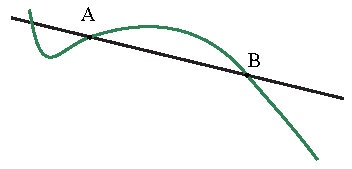
\includegraphics[width=6cm]{./figures/TanL1.pdf}
\caption{割线}
\end{figure}
当 $A$,  $B$ 两点逐渐向 $C$ 点靠近,割线的位置逐渐趋于不变,割线位置的极限\upref{Lim}就叫做曲线在 $C$ 点的切线.

以上对切线的定义中,假设在 $A$,  $B$ 两点靠近 $C$ 点的过程中,割线位置的极限存在.如果这个极限不存在,那么 $C$ 点没有极限.下面举一个简单的例子说明.

\begin{figure}[ht]
\vskip 0pt
\centering
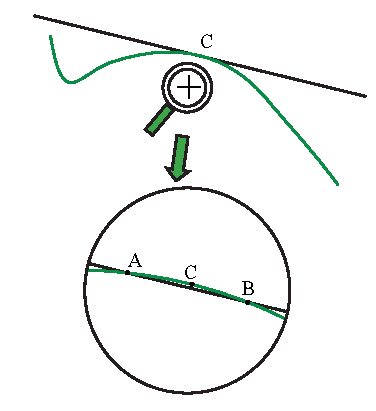
\includegraphics[width=5cm]{./figures/TanL2.pdf}
\caption{割线的极限是切线}
\end{figure}
例如要求正方形一角的切线,用
 $A$,  $B$ 两点接近 $C$ 点,则无论 $AB$ 点
有多么靠近 $C$, 切线的位置还要
取决于 $AB$ 点的具体位置(如右图)
若 $B$ 更接近 $C$, 则直线就更接近竖直
方向.反之直线就更接近水平方向.

% 未完成: 矢量图丢失!

而真正的极限,只取决于点 $A$,  $B$ 都
趋于点 $C$ 的事实,而不要求他们谁
更趋近.所以这个极限不存在.

\rentry{多重极限}














